% Preambolo
\documentclass[12pt,a4paper]{report}

\usepackage[utf8]{inputenc}
\usepackage[T1]{fontenc}
\usepackage[english,italian]{babel}
\usepackage[norules]{frontespizio}
\usepackage{url}
\usepackage{setspace}
\usepackage{graphicx}
\usepackage{listings}

\newcommand{\vir}[1]{``#1''}

% Documento
\begin{document}
\doublespacing
\frenchspacing

% Frontespizio
\begin{frontespizio}
	\Istituzione{Università di Pisa}
	\Logo[6cm]{logo}
	\Dipartimento{Informatica}
	\Corso[Laurea triennale]{Informatica}
	\Annoaccademico{2013--2014}
	\Titoletto{Tesi di laurea}
	\Titolo{Implementazione di un sistema operativo \\ UNIX-like basato su microkernel}
	\Candidato[452264]{Andrea Orrù}
	\Relatore{Antonio Cisternino}
	\Rientro{1.5cm}
\end{frontespizio}

% Abstract
\renewcommand{\abstractname}{Abstract}
\begin{abstract}
	In questa tesi presenteremo \emph{Utopia}, un sistema operativo \emph{UNIX-like} basato su \emph{microkernel}.
	Partiremo da una presentazione generale dei sistemi operativi, descrivendo le motivazioni
	alla base della loro esistenza, e le funzionalità che essi forniscono solitamente.
	Vedremo poi le varie forme in cui questo insieme di funzioni può essere realizzato.
	Infine discuteremo le scelte implementative relative al caso particolare di Utopia.
\end{abstract}

% Indice
\tableofcontents


% Introduzione
\chapter*{Introduzione}
\addcontentsline{toc}{chapter}{Introduzione}
	Il ruolo del sistema operativo (\emph{SO}) è quello di gestire le risorse hardware del calcolatore, fornendo ai programmi
	un'astrazione della macchina sulla quale vengono eseguiti. Il SO si pone dunque come intermediario fra applicazioni e
	hardware della macchina, di solito incapsulando funzioni di I/O\footnote{Input/Output}, gestione della memoria etc.
	in delle \emph{syscall}, e interrompendo liberamente (\emph{preemption}) l'esecuzione dei processi.
	
	Nel linguaggio comune si utilizza spesso la locuzione \emph{sistema operativo} comprendendo con questa definizione tutta
	una serie di applicazioni e funzionalità accessorie come l'interfaccia (grafica o testuale) e le utilità di sistema.
	Queste entità ricoprono però un altro ruolo: quello di intermediario fra gli utenti e il \vir{vero} SO.
	Per questo motivo, nel seguito si parlerà di sistema operativo solo come interfaccia tra hardware e software.\\
	
	L'esistenza dei moderni sistemi operativi è giustificata da necessità di comodità, efficienza e sicurezza.
	
	Comodità, perché la presenza di una API\footnote{Application Programming Interface} unica e coerente per comunicare con
	la grande varietà di hardware esistente libera lo sviluppatore di applicazioni dall'onere della programmazione a basso livello.
	
	Efficienza, perché alternare opportunamente l'esecuzione dei processi consente di riempire i tempi morti della CPU in cui
	i programmi attendono i risultati delle operazioni di I/O, oltre a renderne possibile l'esecuzione concorrente.
	
	Sicurezza, perché delegando la gestione della memoria al sistema operativo, ogni applicazione vive in un suo
	\emph{virtual address space}\footnote{Spazio di indirizzamento virtuale. Ogni processo vede la memoria come se fosse
	l'unico processo in esecuzione.} e non può essere influenzata da altri programmi malfunzionanti, o peggio maliziosi.\\
	
	In questa tesi è mostrato lo sviluppo di un sistema operativo multi-threading minimale ma sufficientemente evoluto
	da comprendere i \emph{driver} per le periferiche di base e consentire il porting della libreria del C e di alcune applicazioni.
	La struttura della tesi è la seguente:


% Capitoli
\chapter{Storia dei sistemi operativi}
	Nei primi calcolatori, per svolgere il proprio compito ogni programma necessitava di propri driver per le periferiche.
	Il crescente livello di complessità delle macchine e delle applicazioni ha man mano reso necessario lo sviluppo dei sistemi operativi.
	
	\section{Batch processing}
		Negli anni 50, \emph{mainframe} che occupavano intere stanze venivano programmati tramite interruttori su enormi pannelli di controllo.
		Più avanti l'introduzione delle \emph{schede perforate} permise di disaccoppiare le fasi di sviluppo
		ed esecuzione, ma soltanto un utente alla volta poteva usufruire della macchina e solo per il periodo di tempo assegnatogli.
		Il calcolatore poteva eseguire soltanto un programma per volta, fino alla sua terminazione.
		
		Questi computer erano del tutto sprovvisti di sistemi operativi. In principio il codice per il controllo della macchina doveva
		essere integrato in ciascun programma, ma a seguito dello sviluppo di \emph{assembler} e \emph{compilatori} divenne
		possibile scrivere delle librerie contenenti funzionalità standard per le operazioni di I/O.
		Questi set di funzioni possono essere considerati i primi antenati dei moderni SO.
		
		In seguito, con l'invenzione dei \emph{batch} di schede perforate, i computer divennero in grado di eseguire
		code di \emph{job} in sequenza, automatizzandone il caricamento. Parallelamente, quelle che prima erano
		solo collezioni di funzioni divennero dei \emph{monitor}, programmi avviati all'accensione della macchina e
		residenti in background. Essi si occupavano di caricare, avviare, monitorare i job e riassegnare le risorse
		hardware al termine di ciascuna esecuzione.
		
		Il primo sistema operativo ad essere utilizzato in ambienti di lavoro reali fu GM-NAA I/O, prodotto
		nel 1956 dalla divisione di ricerca della General Motors per l'IBM 704.
		
	\section{Multiprogrammazione e time sharing}
		Man mano che la potenza computazionale dei computer cresceva, diminuendo i tempi di esecuzione dei job, si faceva
		percentualmente sempre più importante la durata dei tempi morti. Anche se l'introduzione del batch processing aveva
		ridotto drasticamente i tempi di attesa fra un job e il successivo, essa non poteva far nulla per sfruttare gli intervalli
		temporali in cui il programma era in attesa delle lente periferiche di I/O, come le stampanti.
		
		Per ottimizzare l'utilizzo delle risorse fu concepito il concetto di \emph{multiprogrammazione}: diversi job
		vengono caricati sulla memoria del calcolatore; quando uno di loro raggiunge un'istruzione che richiede
		l'attesa di una periferica, lo stato del processo in esecuzione viene salvato e viene data a un altro job
		la possibilità di essere eseguito (\emph{context switch}).
		
		Un ulteriore passo avanti fu compiuto quando ci si rese conto che un singolo utente non poteva sfruttare
		appieno le risorse della macchina. Per consentire a più utenti di interagire contemporaneamente col calcolatore
		furono dunque progettati dei terminali, collegati al computer centrale, che fungevano da interfaccia.
		
		Per rendere possibile questa modalità di utilizzo, che richiede l'esecuzione virtualmente simultanea di
		più programmi, fu introdotta la tecnica del \emph{time sharing}. L'idea alla base del suo funzionamento
		è quella di assegnare brevissimi intervalli di tempo di esecuzione a ciascun processo, così che l'utente
		umano abbia l'illusione che siano eseguiti tutti contemporaneamente.
		
		La tecnica del time sharing comportava un \emph{overhead} affatto trascurabile per i calcolatori dell'epoca.
		Bisogna infatti attendere la fine del 1961 perché veda la luce CTSS\footnote{Compatible Time-Sharing System},
		il primo sistema operativo a fornirne un'implementazione funzionante.
		
		Nel 1964 l'IBM tentò per la prima volta un'opera di unificazione, sviluppando un SO per la sua serie di
		calcolatori System/360, che utilizzavano tutti lo stesso set di istruzioni e la stessa architettura di I/O.
		Fu originariamente concepito come un prodotto unico, ma a causa delle differenze fra le varie dotazioni hardware
		venne frammentato in progetti differenti: DOS/360 pensato per le macchine meno potenti, OS/360 in varie edizioni
		con e senza le funzionalità di time sharing.
		
	\section{Minicomputer e UNIX}
		A partire dalla seconda meta degli anni 60, l'uso dei transistor e delle memorie a nucleo magnetico rese
		possibile lo sviluppo di macchine molto più piccole e dai costi molto più contenuti di quelli dei mainframe.
		Esse presero il nome di \emph{minicomputer}. Alcuni dei calcolatori di maggior successo di questa categoria,
		in particolare la serie PDP, furono prodotti dalla DEC.
		
		Fu proprio su e per queste macchine, le PDP-7 prima e la PDP-11 poi, che venne sviluppato \emph{UNIX}, uno
		dei sistemi operativi più innovativi e influenti della storia, i cui principi sono ancora oggi alla base di
		molti dei più importanti OS odierni.
		
		La prima versione di UNIX vide la luce nel 1969 ad opera dei laboratori di ricerca di AT\&T e Bell, nei quali
		lavoravano tra gli altri Ken Thompson e Dennis Ritchie, ideatore del linguaggio di programmazione C.
		Le prime revisioni del sistema furono realizzate direttamente in assembly, ma nel 1972 venne operata
		una riscrittura in C che rese possibile portare UNIX su svariate altre architetture.

		Alcune delle caratteristiche più significative sono l'impiego di un filesystem gerarchico, dei file come strumenti di
		IPC\footnote{Inter-Process Communication} e la presenza di tante piccole utilità di sistema richiamabili da CLI
		\footnote{Command Line Interface} e combinabili tramite \emph{pipe}.
		L'insieme di questi concetti prende il nome di \vir{filosofia UNIX}, descritta come \vir{l'idea che la potenza di un sistema
		derivi più dalla relazione fra i programmi che da i programmi stessi} \cite{Kernighan}.
		
	\section{Home computer e interpreti BASIC}
		Intorno alla seconda metà degli anni 70, la nascita di microprocessori a 8-bit quali il MOS 6502, l'Intel 8080 e lo Zilog Z80
		incoraggiò lo sviluppo di una nuova categoria di calcolatori, dapprima appannaggio dei soli hobbisti, ma ben presto
		destinata a conquistare ampie fascie di mercato.
		
		I cosiddetti \emph{home computer}, come l'Apple II, lo ZX Spectrum o il leggendario Commodore 64, erano equipaggiati
		con quantità minimali di memoria e non possedevano le risorse hardware sufficienti per far girare efficacemente un vero
		e proprio sistema operativo. All'interno della ROM era preinstallato un interprete BASIC che fungeva da interfaccia testuale,
		e i programmi avevano il controllo totale della macchina mentre erano in esecuzione.
		
		\begin{figure}[htbp]
		\centering
		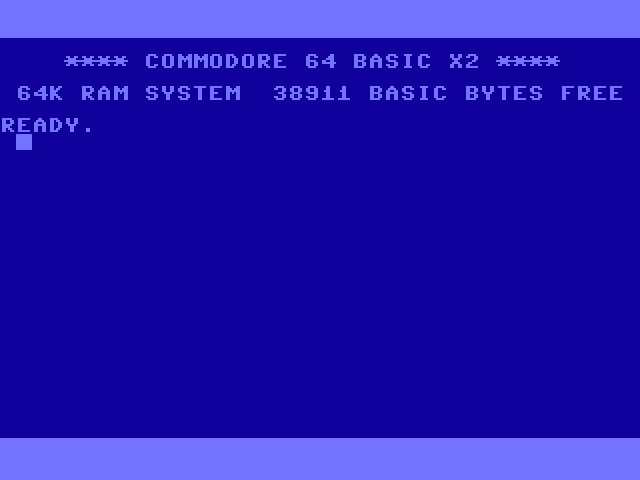
\includegraphics[scale=0.5]{img/commodore64.png}
		\caption{L'interprete BASIC del Commodore 64.\label{fig:commodore64}}
		\end{figure}
		
	\section{Personal computer}
		\subsection{IBM PC e DOS}
			Nel 1981 il colosso IBM, che dominava il settore dei mainframe ma che fino ad allora non si era occupato del mercato
			dei calcolatori domestici, introdusse l'\emph{IBM PC}, costruito attorno al processore a 16-bit Intel 8088 e con una
			architettura aperta e espandibile. Il sistema operativo scelto dall'IBM per pilotare queste macchine fu \emph{MS-DOS}, sviluppato
			dalla Microsoft sulla base di 86-DOS, del quale la società di Bill Gates aveva acquistato i diritti per 50000\$.
		
			Come la maggior parte dei sistemi operativi per home e personal computer del tempo, MS-DOS era monoutente
			e monotask \cite{WIKI_MS-DOS}. Di base forniva un'interfaccia a riga di comando con cui poter gestire i file
			e lanciare i programmi, i quali assumevano però il controllo totale del sistema una volta avviati.
			
		\subsection{Interfacce grafiche: Mac OS e Windows}
			Il primo sistema operativo a rendere popolare il concetto di GUI\footnote{Graphical User Interface} e la metafora del desktop
			fu \emph{Mac OS} \cite{WIKI_MacHistory}, il SO preinstallato sull'Apple Macintosh, lanciato nel 1984.
			La Microsoft collaborò con la Apple per la realizzazione di molte delle applicazioni del Macintosh e, a partire da questa
			esperienza, fece confluire molte delle idee dell'azienda di Cupertino nel proprio sistema operativo, Windows, la cui
			prima versione vide la luce nel 1985.
			Nelle sue prime incarnazioni, Windows non era però un SO \emph{standalone}, bensì un'estensione per MS-DOS,
			col quale condivideva l'assenza di multitasking e i limiti nella gestione della memoria.
	
			\begin{figure}[htbp]
			\centering
			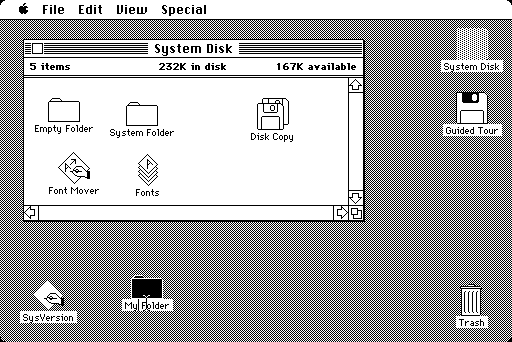
\includegraphics[scale=0.6]{img/macos.png}
			\caption{L'interfaccia grafica della prima versione di Mac OS.\label{fig:macos}}
			\end{figure}
			
		\subsection{L'Intel x86 e il multitasking su PC}
			L'introduzione da parte di Intel dei processori 386, dotati di MMU\footnote{Memory Management Unit} e quindi capaci di fornire a
			livello hardware meccanismi di protezione della memoria, aprì la strada alla realizzazione di sistemi operativi multitasking
			fino ad allora confinati ai costosi mainframe.

\chapter{L'architettura x86}
	In questo capitolo daremo una descrizione sommaria dei processori Intel x86, largamente la più comune nei PC moderni.
	Porremo l'accento in particolare sulle serie a 32-bit (dalla 386 alla 686).
	
	L'obiettivo è di dare al lettore una comprensione dell'architettura sufficiente da poter apprezzare i dettagli implementativi
	illustrati nei capitoli successivi.
	
	\section{Set di istruzioni e registri}
		L'architettura x86 consiste di un set di istruzioni di lunghezza variabile, con un'impronta prevalentemente
		\emph{CISC}\footnote{Complex Instruction Set Computer} e una forte enfasi sulla retrocompatibilità \cite{WIKI_x86}.
		Questo significa che il cuore dell'instruction set è a tutt'oggi quello dei vecchi processori a 16-bit.
		
		Per illustrare questo concetto è significativo l'esempio dei registri (si veda la figura~\ref{fig:gpr}).
		Si consideri il registro AX; è possibile accedere rispettivamente ai suoi 8 bit alti e bassi tramite AH e AL.
		
		Analogamente, sui processori dal 386 in poi, aggiungendo il prefisso \textbf{E} (es. EAX) si accede al corrispondente
		registro a 32-bit, ma è ancora possibile agire sui 16 bit bassi riferendosi a AX.
		
		\begin{figure}[t]
		\centering
		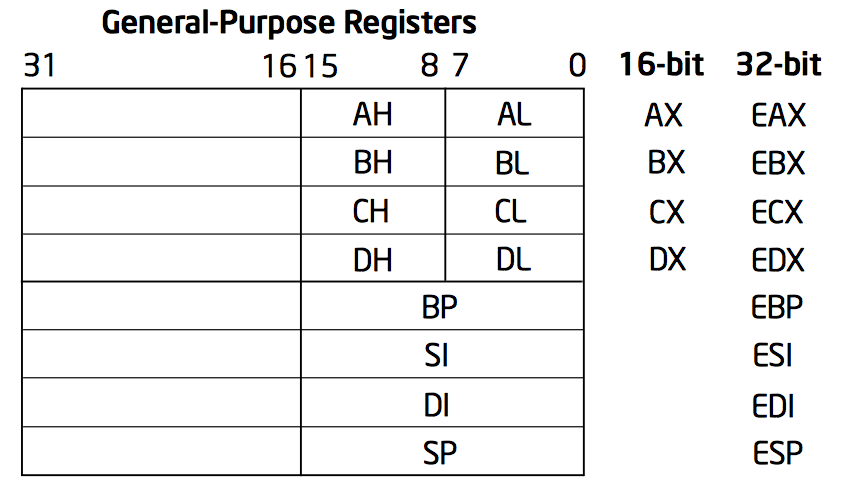
\includegraphics[scale=0.6]{img/gpr.png}
		\caption{I registri \emph{general purpose} dell'architettura x86. \cite{Intel}\label{fig:gpr}}
		\end{figure}

		\begin{figure}[b!]
		\centering
		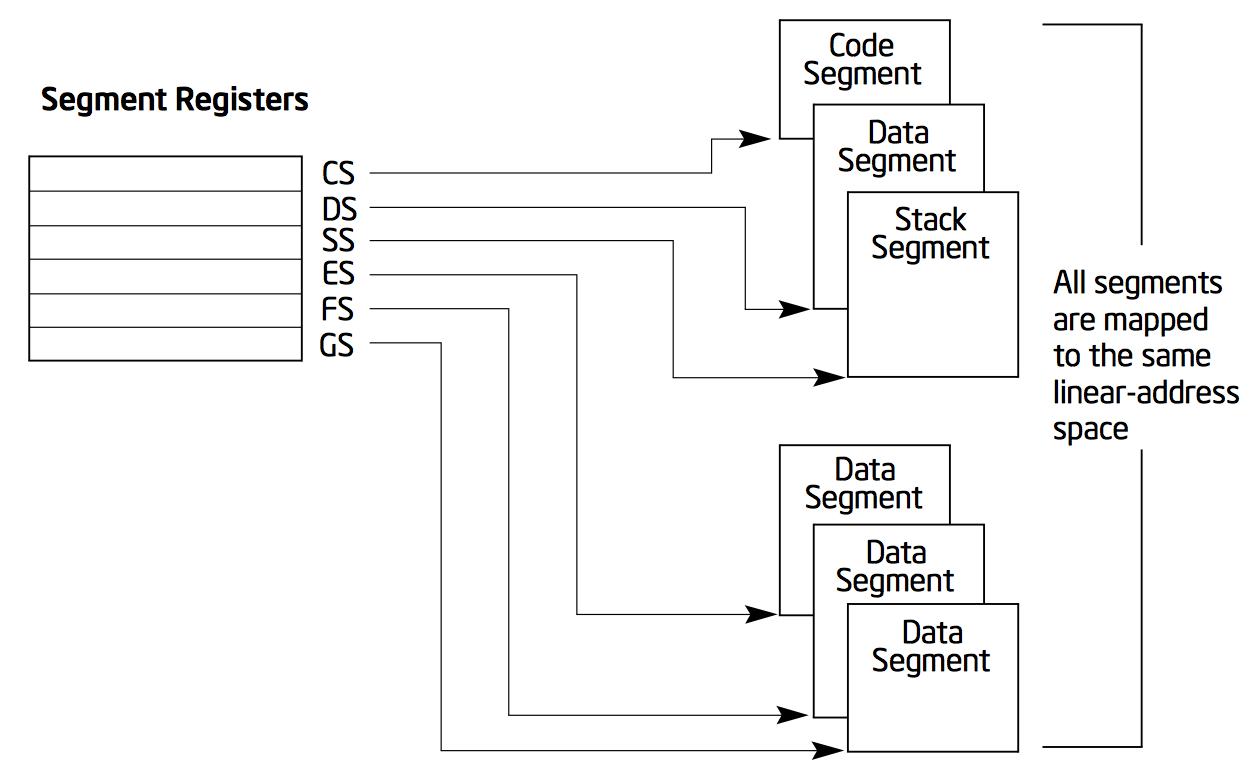
\includegraphics[scale=0.5]{img/segment.png}
		\caption{Registri segmento. \cite{Intel}\label{fig:segment}}
		\end{figure}

	\section{Modalità operative}
		\subsection{Real mode}
			Per le suddette esigenze di retrocompatibilità, tutti i processori x86 (e anche i più moderni x86-64) si avviano
			in modalità 16-bit, che in gergo prende il nome di \emph{real mode}.
			In questo assetto il processore può indirizzare solo 20 bit di memoria (1 MiB), specificati dalla somma fra
			un registro segmento (si veda la figura~\ref{fig:segment}), il cui contenuto viene shiftato di 4 bit verso sinistra,
			e un offset di 16 bit.
		
			In real mode il processore non fornisce alcun meccanismo di protezione della memoria, e il software può
			accedere direttamente alle periferiche hardware e richiamare le routine del \emph{BIOS}\footnote{Basic Input/Output System:
			un insieme di routine software memorizzato in ROM, che fornisce una serie di funzioni di base per l'accesso all'hardware del computer.}
			tramite degli \emph{interrupt software}.
		
		\subsection{Protected mode}
			Inizializzando alcune strutture dati e modificando alcuni registri di controllo si può impostare il processore
			in \emph{protected mode}. In questa modalità i registri segmento non indicano più un indirizzo assoluto,
			ma un indice in una tabella detta \emph{GDT}\footnote{Global Descriptor Table}, che consente di definire
			segmenti di 32-bit (4 GiB) e assegnare loro alcune proprietà.
			
			Fra queste, la più significativa è la possibilità di selezionare uno fra quattro \emph{protection ring} per la
			il segmento, istituendo così dei limiti sugli accessi a determinate zone di memoria.
			Diventa possibile, ad esempio, riservare un segmento di memoria al solo \emph{Ring 0} (l'anello coi privilegi più elevati),
			consentendone l'accesso solo al codice che girà in quella modalità.
			
			Tipicamente, il \emph{kernel} di un sistema operativo gira in Ring 0 (l'unica modalità che ha accesso
			a tutte le risorse del sistema), mentre le applicazioni in Ring 3 (si veda la figura~\ref{fig:ring}).
			
			\begin{figure}[htbp]
			\centering
			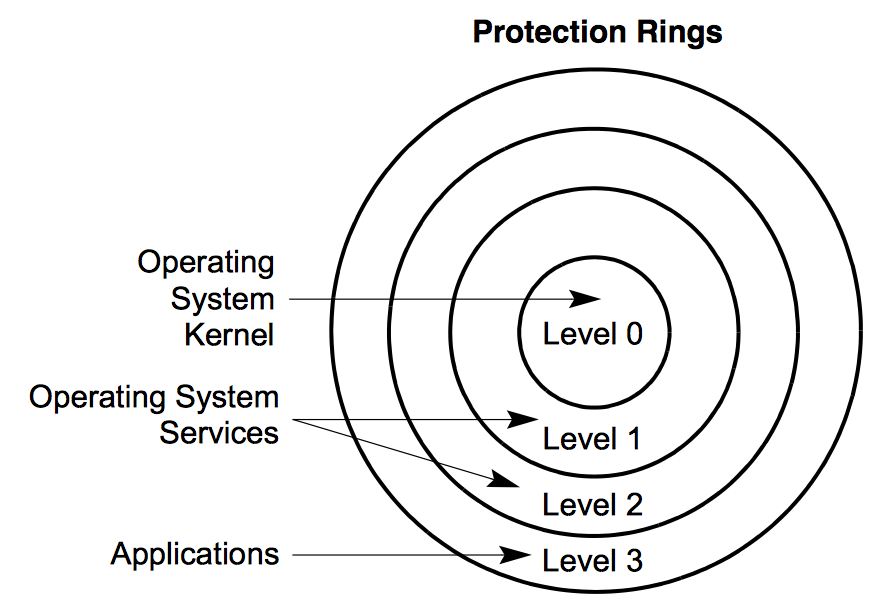
\includegraphics[scale=0.5]{img/ring.png}
			\caption{Anelli di protezione. \cite{Intel}\label{fig:ring}}
			\end{figure}
			
	\section{Paginazione}
		Una delle funzionalità più utili offerte dalla protected mode dal punto di vista dello sviluppo dei sistemi operativi
		è il \emph{paging}, un meccanismo di \emph{memoria virtuale}.
		Quando il paging è attivo, lo spazio di indirizzamento virtuale è diviso in \emph{pagine} di 4 KiB ciascuna.
		Ad ognuna di queste pagine è possibile assegnare un indirizzo di memoria fisica, riempendo delle opportune
		strutture dati interpretate dalla MMU\footnote{Memory Management Unit}, dette \emph{page tables}.
		
		\begin{figure}[htbp]
		\centering
		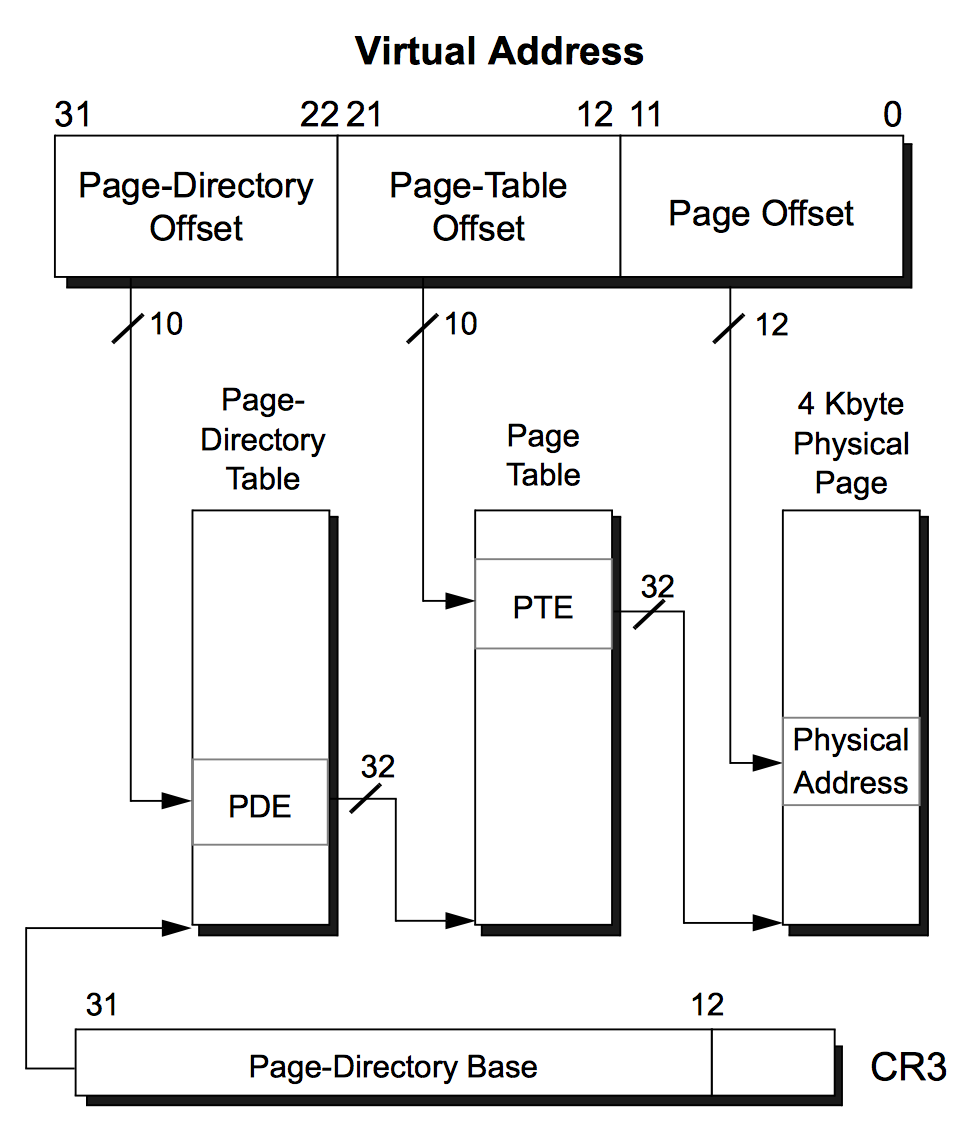
\includegraphics[scale=0.7]{img/translation.png}
		\caption{Traduzione degli indirizzi virtuali in indirizzi fisici. \cite{AMD}\label{fig:translation}}
		\end{figure}
		
	\section {Interrupt e I/O}
				
\chapter{Struttura dei sistemi operativi}
	In questo capitolo forniremo una descrizione dettagliata delle componenti e dell'organizzazione di un sistema operativo e
	delle possibili soluzioni implementative. Illustreremo e metteremo poi a confronto due casi concreti, Linux e Windows.	

\chapter{L'implementazione di Utopia}
			
						
% Bibliografia
\begin{thebibliography}{}
	\bibitem{Silberschatz}
		Silberschatz A., Galvin P. B., Gagne G.,
		\emph{Operating System Concepts}.
		Wiley,
		9th Edition,
		2012.
	\bibitem{Kernighan}
		Kernighan B., Pike R.,
		\emph{The UNIX Programming Environment}.
		Prentice Hall,
		1984.
	\bibitem{Intel}
		\emph{Intel 64 and IA-32 Architectures Software Developer’s Manual}.
		Intel,
		February 2014.
	\bibitem{AMD}
		\emph{AMD64 Architecture Programmer’s Manual Volume 2: System Programming}.
		AMD,
		May 2013
	\bibitem{WIKI_OS}
		Wikipedia, Operating system.
		\emph{\url{http://en.wikipedia.org/wiki/Operating_system}}
	\bibitem{WIKI_OSHistory}
		Wikipedia, History of operating systems.
		\emph{\url{http://en.wikipedia.org/wiki/History_of_operating_systems}}
	\bibitem{WIKI_MS-DOS}
		Wikipedia, MS-DOS.
		\emph{\url{http://it.wikipedia.org/wiki/MS-DOS}}
	\bibitem{WIKI_MacHistory}
		Wikipedia, History of Mac OS.
		\emph{\url{http://en.wikipedia.org/wiki/History_of_Mac_OS}}
	\bibitem{WIKI_x86}
		Wikipedia, x86.
		\emph{\url{http://it.wikipedia.org/wiki/x86}}
\end{thebibliography}

\end{document}
